%!TEX root = bambi-thesis.tex
This chapter begins with a theory digression about the topic of Coverage Path Planning. Then the algorithm chosen for the application in this thesis is explained in details and finally the ROS implementation of the algorithm is presented and discussed.
\section{Theory Background} % (fold)
\label{sec:theory_background}
\textit{Coverage path planning} (CPP) is the problem of finding a trajectory for a mobile robot such that a target area is completely swept by the sensor footprint. In the following section it is first presented the conventional CPP algorithms in use for mobile robots. Later, the focus moves more specifically over aerial application showing some previous work regarding this topic.

\subsection{Coverage Path Planning for Mobile Robots} % (fold)
\label{sub:coverage_path_planning_for_mobile_robots}
The problem of finding an optimal coverage path, even for a simple polygon, is classified as NP-hard \footnote{NP-hard problems are problems for which there is no known polynomial algorithm, so that the time to find a solution grows exponentially with problem size. Although it has not been definitively proven that, there is no polynomial algorithm for solving NP-hard problems, many eminent mathematicians have tried and failed.} \cite{ARKIN200025}. Hence, existing approaches try to find an approximate solution which fits at best the specific application requirements. For 2D coverage, some methods decompose the target area into simpler polygons and for each compute the coverage path. Other methods use a grid-based representation which leads to an approximate coverage. Finally, closed-loop control methods avoid the needs of an a priori representation of the target region.

\subsubsection{Exact Cellular Decomposition} % (fold)
\label{ssub:exact_cellular_decomposition}
One of the main approach in area coverage path planning is based on the divide-and-conquer strategy.
In this method the target area is decomposed in simple regions called cells. Since all cells have a simple structure, each can be covered with simple motions such as back-and-forth motion as in \autoref{fig:lawnmower-pattern}. This kind of motion is called \textit{Lawnmower pattern}. Once the robot visits all cell, coverage is achieved.\par
\textit{Trapezoidal decomposition} is the most popular cell decomposition. This decomposition relies heavily on the polygonal representation of the planar configuration space \cite{book:655068}. Cells are in fact obtained simply by sweeping a vertical line,termed as \textit{slice}, through the 2D plane and, upon reaching each vertex of the environment polygon, the required edges are added to create trapezoids (see \autoref{fig:trapezoidal-decomposition}). Two cells sharing a common boundary are defined as adjacent and accordingly an adjacent graph is produced. At this point the strategy consist in finding the exhaustive walk which visits all cells and minimizes the cost of traveling between them.
An important factor in finding an efficient path is the choice of the slice direction when decomposing the target area as analyze by Oksane \cite{TrapezoidalDecompCPP}. In his work, he performed a local optimization to find the direction for the sweeping line which minimize trajectory length and the number of turnings. \par
\begin{figure}[ht]
    \centering
    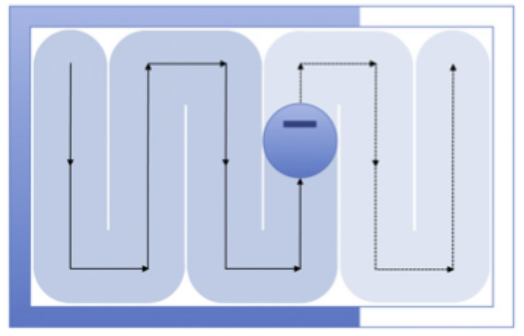
\includegraphics[width=0.4\textwidth]{figures/C3/LawnmowerPattern.png}
    \caption{Lawnmower pattern}
    \label{fig:lawnmower-pattern}
\end{figure}
\begin{figure}[ht]
    \centering
    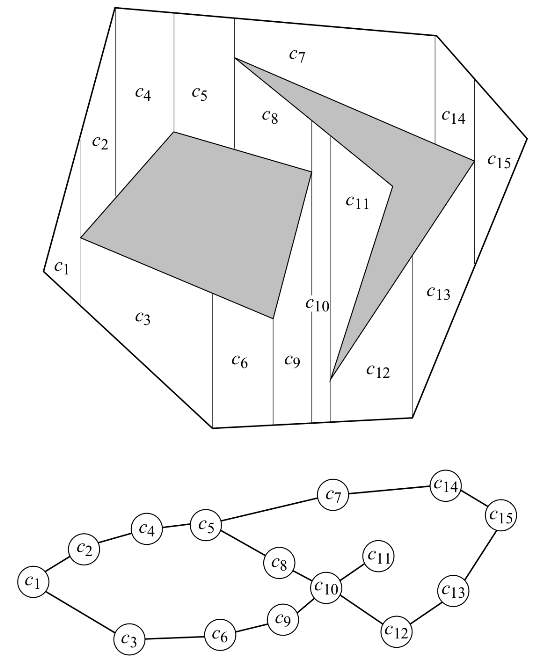
\includegraphics[width=0.4\textwidth]{figures/C3/TrapezoidalDecomposition.png}
    \caption{Trapezoidal decomposition and adjacent graph \cite{book:655068}}
    \label{fig:trapezoidal-decomposition}
\end{figure}
In trapezoidal approach many neighbor cells could be merged together into one cell resulting
in a shorter coverage path. In the left hand side of \autoref{fig:trapezoidal-boustrophedon} the robot needs to make one additional lengthwise motion to cover the remaining portion of the trapezoidal cell.
Following this idea, Choset proposed in \cite{Choset-1997-16422} an enhancement of the trapezoidal decomposition method, the \textit{Boustrophedon cellular decomposition} designed with the aim to minimize the path length by generating bigger cells.
\begin{figure}[ht]
    \centering
    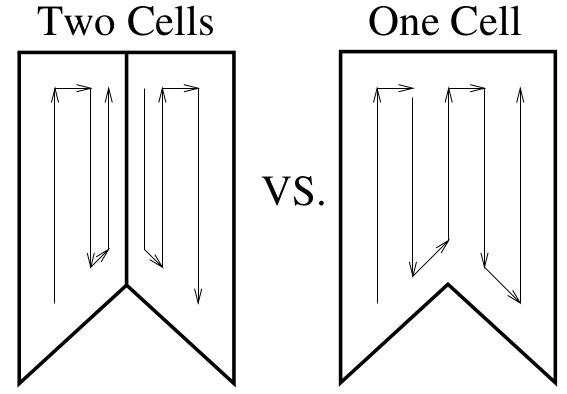
\includegraphics[width=0.3\textwidth]{figures/C3/trapezoidalVsBoustrophedon.png}
    \caption{Fewer cells is better}
    \label{fig:trapezoidal-boustrophedon}
\end{figure}
The boustrophedon decomposition is formed similarly to trapezoidal, but by considering only the vertices at which the slice can be extended both up and down in the free space (see \autoref{fig:boustrophedon-decomposition}). Such vertices are called \textit{critical points}. As before, by visiting all the nodes in the adjacency graph the area is covered completely.\par
\begin{figure}[ht]
    \centering
    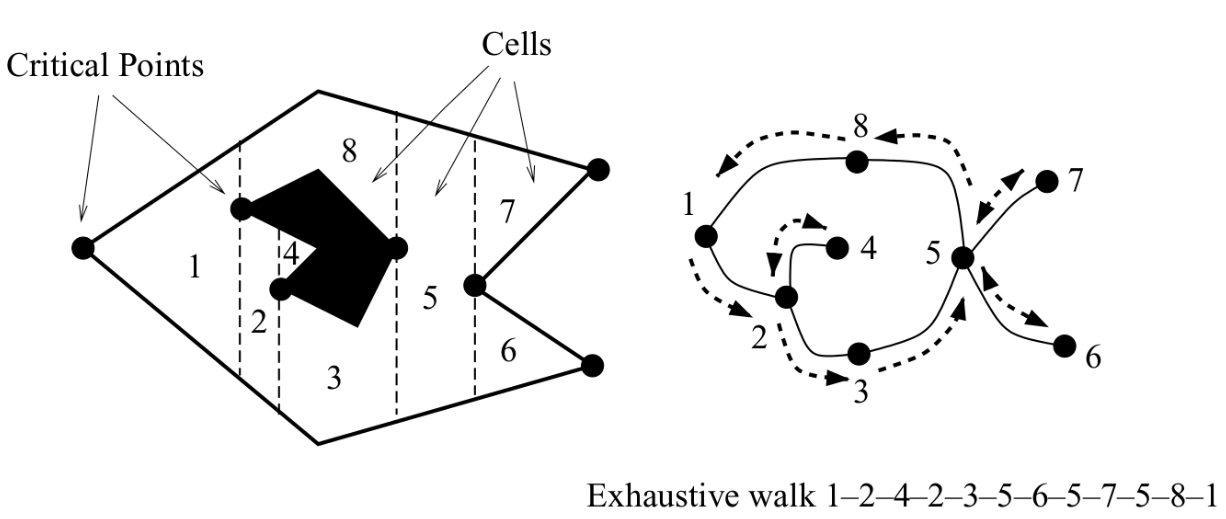
\includegraphics[width=0.65\textwidth]{figures/C3/boustrophedonDecomposition.png}
    \caption{Fewer cells is better}
    \label{fig:boustrophedon-decomposition}
\end{figure}
In summary, exact cellular decomposition guarantees a complete coverage of the target area. A bigger drawback to the trapezoidal method is that it fundamentally requires a polygonal workspace, which is not a realistic assumption for many applications. To overcome this limitation the boustrophedon decomposition was designed.
% subsubsection exact_cellular_decomposition (end)

\subsubsection{Grid-based Methods} % (fold)
\label{ssub:grid_based_methods}
Another largely used method in coverage path planning divides the environment in a collection of grid cells of the same shape. Each cell is marked as empty or occupy according to the presence of obstacle in that location. This will produce an \textit{approximate cellular decomposition} as the obstacles are represented by grid cells.
The algorithms using this grid-based representation should plan a path which visit all the empty cells of the grid minimizing the traveling cost. Primitive criteria could be to avoid revisiting cells and to move from adjacent cells only. Two interesting algorithms have been developed for this scope: The \textit{Wave-front} method \cite{Zelinsky93planningpaths} and \textit{Minimum-Spanning-Tree} (MST) method \cite{Gabriely2001}.\par
The \textit{Wave-front} method is based upon distance transform (DT) path planning methodology. This approach considered the task of path planning to finding paths from the goal location back to the start location. The path planner propagates a distance wavefront through all free space grid cells starting from the goal cell. The distance wave front flows around obstacles and eventually through all free space in the environment.\\
 \textit{"For any starting point within the environment representing the initial position of the mobile robot, the shortest path to the goal is traced by walking down hill via the steepest descent path. If there is no downhill path, and the start cell is on a plateau then it can be concluded that no path exists from the start cell to the goal cell i.e. the goal is unreachable"} \cite{Zelinsky93planningpaths}.\\
One significant advantage that distance transform path planning has over other path planning methods is that it can easily be induced to exhibit different types of robot navigation behaviors. In addition to the "optimum" i.e. shortest path behavior it is possible to have the "complete coverage" behavior. To achieve the complete coverage
path planning behavior, instead of descending along the path of steepest descent to the goal, the robot follows the
path of steepest ascent. In other words the robot moves away from the goal keeping track of the cells it has visited. The robot only moves into a grid cell which is closer to the goal if it has visited all the neighbouring cells which lie further away from the goal. An example of the complete coverage path is shown in \autoref{fig:wavefront}.
\begin{figure}[ht]
\centering
\begin{subfigure}{.5\textwidth}
  \centering
  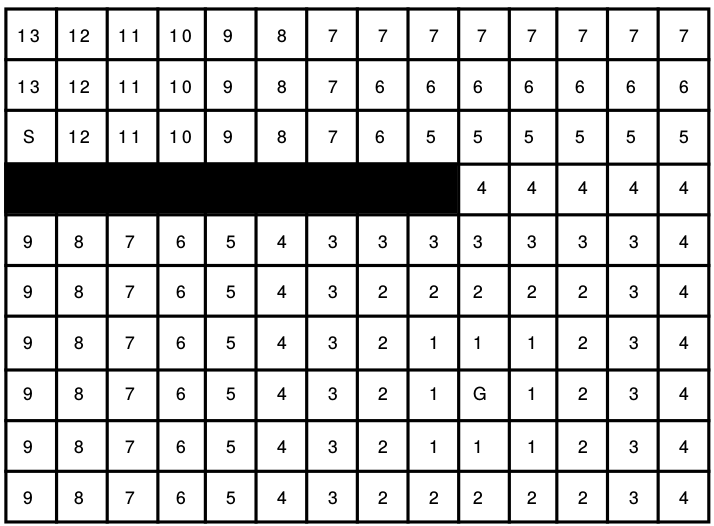
\includegraphics[width=.9\linewidth]{figures/C3/wavefrontGrid.png}
  \caption{Distance waveform grid}
\end{subfigure}%
\begin{subfigure}{.5\textwidth}
  \centering
  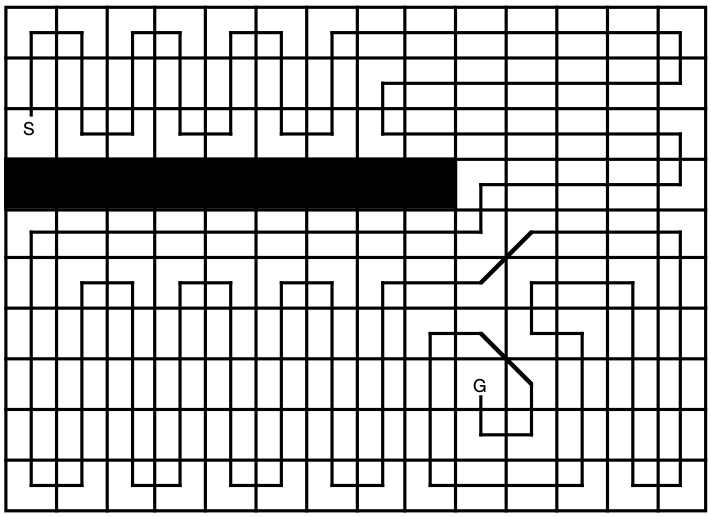
\includegraphics[width=.9\linewidth]{figures/C3/wavefrontCPath.png}
  \caption{Path of complete coverage}
\end{subfigure}
\caption{Wavefront method \cite{Zelinsky93planningpaths}}
\label{fig:wavefront}
\end{figure}
The pseudocode to obtain such behavior is listed in \autoref{alg:Wavefront-distance}.\todo{valutare se mettere l'algoritmo qui o dopo}
A nice feature of this approach is that it is possible to set both starting and goal position. This comes in handy in cleaning or lawn mowing application. However, in some case this method can not avoid revisiting cells. Another shortcoming it is worth to highlight is the high number of turn in the coverage path. This is because the path follows the "spiral" of the distance transform wave front that radiates from the goal. A solution to this problem as will be presented in the next sections, could be to take into account other factors than only the distance from the goal.\par
\begin{algorithm}
	\SetKwData{SCell}{startCell}\SetKwData{CCell}{currentCell}\SetKwData{Cell}{cell}\SetKwData{Stop}{stop}\SetKwData{NeighborCell}{neighborCell}
	\SetKwData{Left}{left}\SetKwData{This}{this}\SetKwData{Up}{up}
	\SetKwFunction{Union}{Union}\SetKwFunction{FindCompress}{FindCompress}
	\SetKwInOut{Input}{input}\SetKwInOut{Output}{output}

	\Input{A matrix $M$ representing the grid}
	\Output{A matrix $M$ filled with Distance Transformation}
	\BlankLine
	\SCell $\leftarrow$ \CCell \;
	\ForAll{cells of $M$}{
		 \Cell $\leftarrow$ $NotVisited$\;	
	}
	\Repeat{\Stop is true}{
		Find \textit{unvisited Neighboring cell} with highest $DT$\;
		\If(\tcc*[h]{Goal reached}){No \NeighborCell found}{
			\CCell $\leftarrow$ $Visited$\;
			\Stop $\leftarrow$ true\;
		}
		\If{\NeighborCell DT $\leq$ \CCell DT}{
			\CCell $\leftarrow$ $Visited$\;
		}
		\CCell $\leftarrow$ \NeighborCell\;
	}
\caption{CPP algorithm based on Distance Wavefront}
\label{alg:Wavefront-distance}
\end{algorithm}
The \textit{Minimum-Spanning-Tree} (MST) method only considers the cells that are completely unoccupied by obstacles [74]. First, a grid with cells 4 times the robot sensor footprint is constructed. Then a graph is created by representing each cell with a node and connecting two nodes if they are neighbor cells. The minimum spanning tree of this graph then is computed. In order to achieve complete coverage of the environment the robot circumnavigates the spanning tree visiting quadrants of the cells as shown in \autoref{fig:MST-path}. Unlike the wave-front method, this algorithm never revisits a cell and hence produces an optimal solution in terms of path length. 
\begin{figure}[ht]
    \centering
    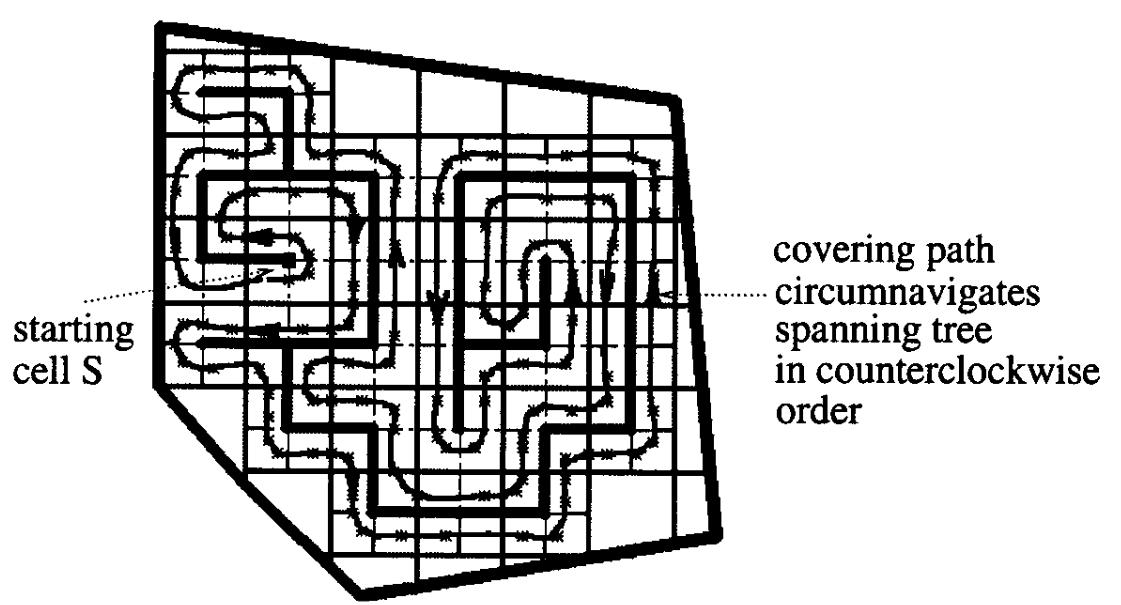
\includegraphics[width=0.65\textwidth]{figures/C3/MST-path.png}
    \caption{Minimum Spanning Tree method}
    \label{fig:MST-path}
\end{figure}
% subsubsection grid_based_methods (end)


% subsection coverage_path_planning_for_mobile_robots (end)
\subsection{Aerial Coverage using UAVs} % (fold)
\label{sub:aerial_coverage_using_uavs}


% The general CPP methods introduced in Chapter 2.2.1 have been applied directly to aerial coverage often in an offline setting. In these works, the target area is specified as a polygon or grid with GPS coordinates of the polygon nodes or grid center. It is usually assumed that the UAV is flying at an altitude which is safe and hence there is no risk of colliding with an obstacle. However sometimes some parts of the environment are treated as no-flying zones which should be avoided by the UAV. Therefore in CPP for UAVs, these subregions are dealt with as obstacles. Another type of region that might be present in aerial coverage is uninteresting regions. Flying in these regions is allowed but does not contribute to the coverage goal i.e. covering them is of no value. For example in a outdoor crop mapping task with a quadrotor, covering the lake is unnecessary but flying over it (for example to reach the other side of the lake) is allowed.\\
% As mentioned before, due to the very short flight time of UAVs, generating efficient coverage paths is useful. To reach efficiency, existing methods try to avoid unnecessary coverage, i.e. they try to minimize the overlap in the sensor footprint along the produced trajectory. This goal will consequently reduce the path length. Another element considered by some existing methods is to minimize the number of turns in the flight trajectory. Reducing the number of turnings will consequently produce trajectories that consist of long straight stripes, as is the case in Lawnmower pattern. Therefore, when a robot follows the trajectory it can maintain a constant velocity in a large part of the coverage path and it only accelerates or de-accelerates when it is turning. The overall outcome is less power consumption. Such efficient coverage trajectories can be planned offline when the environment is known a priori. Some of these methods, aimed for aerial coverage, are presented in the following section which includes planning for both single and multi-robot systems. However, when no prior knowledge about the target area is available, the planning has to be done online based on the real-time sensory data.\\
% In the following, we present the existing methods of coverage trajectories planning for unmanned aerial vehicles. We partition the approaches into two main groups: a) methods that precompute the trajectory based on a priori knowledge of the environment and b) methods that adaptively re-plan the trajectory based on on-line sensory data.
 % subsection aerial_coverage_using_uavs (end)

\subsection{Flight Altitude} % (fold)
\label{sub:flight_altitude}
How to compute the required flight altitude (resolution + sensor footprint + required photo overlap). Some calculation will be listed.
% subsection flight_altitude (end


% section theory_background (end)

\section{Proposal Solution} % (fold)
\label{sec:proposal_solution}

Abbiamo scelto il wavefront perche' oltre ad essere abbastanza efficente computazionalmente permette di tenere conto di diverse cost function (diverse priorita' come ad esempio variazioni di altitudine, minor number of turns, ecc...)]
% section proposal_solution (end)


\section{Implementation in ROS} % (fold)
\label{sec:implementation_in_ros}


% section cpp_algorithms (end)